\section{ECAPA-TDNN}
Desplanques et al. \cite{desplanques2020} proposed ECAPA-TDNN architecture that significantly outperformed state-of-the-art TDNN based systems on the VoxCeleb test sets and the 2019 VoxCeleb Speaker Recognition Challenge \cite{chung2019voxsrc2019voxcelebspeaker}. Notably, the architecture was also recommended by the Deep Noise Suppression challenge in 2023 \cite{dubey2023} for its robustness and efficiency in speaker embedding tasks. It was also used by the state-of-the-art TEA-PSE 3.0 \cite{ju2023teapse30tencentetherealaudiolabpersonalized} model which won the first place in the 2023 Deep Noise Suppression Challenge.

The authors proposed several enhancements to the successful Time Delay Neural Network (TDNN) architecture, drawing on recent advancements in face verification and computer vision. Traditionally, TDNN uses statistics pooling to convert variable-length utterances into fixed-length speaker characterizing embeddings.

Firstly, the initial frame layers were restructured into 1-dimensional Res2Net modules \cite{Res2Net} with impactful skip connections. These modules also incorporate Squeeze-and-Excitation (SE) blocks \cite{Squeeze-and-Excitation}, similar to those in SE-ResNet, to explicitly model channel interdependencies. The SE blocks expand the temporal context of the frame layer by rescaling the channels based on the recording's global properties.

Secondly, recognizing that neural networks learn hierarchical features, with each layer capturing different levels of complexity, the authors aggregated and propagated features from various hierarchical levels to leverage this complementary information.

Finally, they enhanced the statistics pooling module with channel-dependent frame attention. This improvement allows the network to focus on different subsets of frames during each channel's statistics estimation.

\subsection{Model Architecture}

An overview of the complete architecture can be shown as in Figure \ref{fig:ecapa-tdnn}.

\subsubsection{Context-dependent statistics pooling}
Recent x-vector architectures employed soft self-attention for calculating weighted statistics in the temporal pooling layer. The success of multi-headed attention demonstrated that specific speaker properties could be extracted from different sets of frames. Building on these results, the authors proposed extending this temporal attention mechanism to the channel dimension. This extension allowed the network to focus on speaker characteristics that manifested at different time instances, such as the distinct properties of vowels versus consonants.

\subsubsection{Res2Blocks}
The temporal context of frame layers in the original x-vector system was limited to 15 frames. Recognizing that a wider temporal context could be beneficial, the authors suggested rescaling frame-level features based on the global properties of the recording, similar to the global context in the attention module described above. For this purpose, the authors introduced 1-dimensional Squeeze-Excitation (SE) blocks, a technique proven successful in modeling global channel interdependencies in computer vision.

Integrating the 1-dimensional SE-block into the x-vector architecture could be done in various ways, with the most straightforward method being their placement after each dilated convolution. However, the authors aimed to combine these blocks with the advantages of residual connections while minimizing the increase in total parameters compared to baseline systems. The SE-Res2Block, depicted in Figure \ref{fig:se-res2block}, met these requirements. It included dilated convolutions flanked by dense layers with a context of 1 frame each. The first dense layer reduced the feature dimension, while the second restored it to the original dimension. This was followed by an SE-block that scaled each channel, with the entire unit enclosed by a skip connection.

The use of these traditional ResBlocks makes it easy to incorporate advancements concerning this popular computer vision architecture. The recent Res2Net module, for example, enhances the central convolutional layer so that it can process multi-scale features by constructing hierarchical residual-like connections within. The integration of this module improved the performance, while significantly reducing the number of model parameters.

\begin{figure}[ht]
    \centering
    \begin{minipage}{0.35\textwidth}
        \centering
        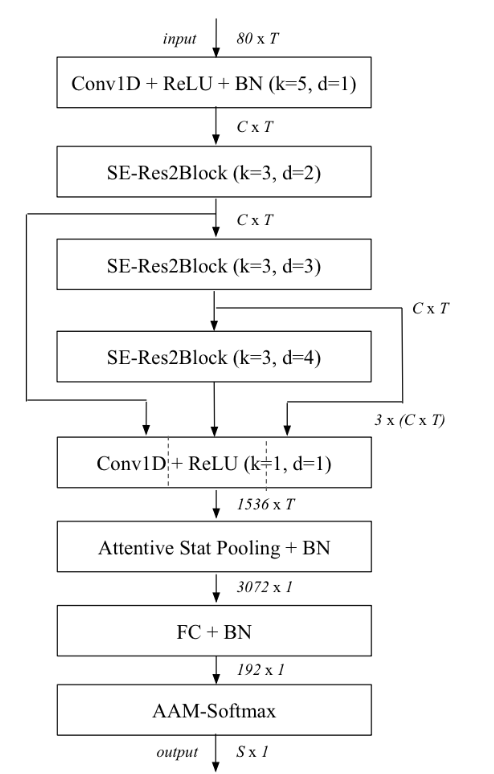
\includegraphics[width=\textwidth]{images/related_work/ecapa-tdnn/SE-Res2Block.png}
        \captionsetup{width=.9\linewidth}
        \caption{The SE-Res2Block of the ECAPA-TDNN architecture.}
        \label{fig:se-res2block}
    \end{minipage}\hfill
    \begin{minipage}{0.35\textwidth}
        \centering
        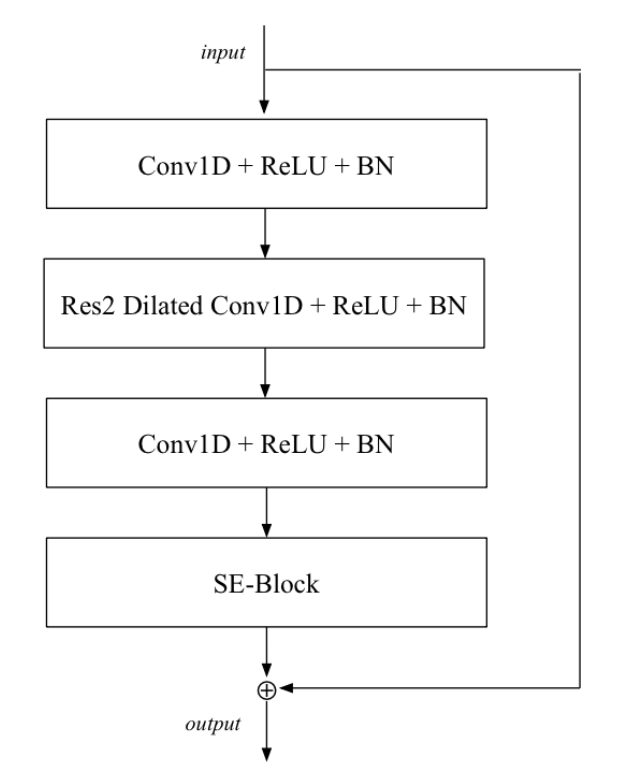
\includegraphics[width=\textwidth]{images/related_work/ecapa-tdnn/ECAPA-TDNN.png}
        \captionsetup{width=.9\linewidth}
        \caption{Network topology of the ECAPA-TDNN.}
        \label{fig:ecapa-tdnn}
    \end{minipage}
\end{figure}

\subsubsection{Hierarchical feature aggregation}
The original x-vector system only uses the feature map of the last frame-layer for calculating the pooled statistics. Given the hierarchical nature of a TDNN, these deeper level features are the most complex ones and should be strongly correlated with the speaker identities. However, the authors argued that the more shallow feature maps can also contribute towards more robust speaker embeddings. For each frame, their proposed system concatenates the output feature maps of all the SE-Res2Blocks. After this Multi-layer Feature Aggregation (MFA), a dense layer processes the concatenated information to generate the features for the attentive statistics pooling. 

Another, complementary way to exploit multi-layer information is to use the output of all preceding SE-Res2Blocks and initial convolutional layer as input for each frame layer block. The authors implemented this by defining the residual connection in each SE-Res2Block as the sum of the outputs of all the previous blocks. They opted for a summation of the feature maps instead of concatenation to restrain the model parameter count. The final architecture without the summed residual connections is shown in Figure \ref{fig:ecapa-tdnn}.

\subsection{Experimental Setup}
The training was done using the development set of the VoxCeleb2 dataset with a split of 98\% for training data and reserving a small subset of 2\% as a validation set for hyperparameter optimization. Various data augmentation techniques were introduced to the VoxCeleb2 dataset, including:

\begin{itemize}
    \item Kaldi recipe \cite{snyder2019}
    \item Babble effect and extra noises from MUSAN dataset \cite{musan}
    \item Reverberation effect
    \item Open-source SoX library (tempo up, tempo down)
    \item FFmpeg library for alternating opus and acc compression
\end{itemize}

The input features are 80-dimensional MFCCs from a 25 ms window with a 10 ms frame shift. Two second random crops of the MFCCs feature vectors are normalized through cepstral mean subtraction and no voice activity detection is applied.

The models are trained using batch size of 128 and with a learning rate varying between $1 \times 10^{-8}$ and $1 \times 10^{-3}$ using the triangular2 policy and Adam optimizer \cite{kingma2017adam}. Each cycle has 130k iterations. To prevent overfitting, weight decay on all weights were applied with $2 \times 10^{-5}$, except for the AAM-softmax weights, which used $2 \times 10^{-4}$.

The dimension of the bottleneck in the SE-Block and the attention module is set to 128. The scale dimension in the Res2Block is set to 8. The number of nodes in the final fully-connected layer is 192.

Speaker embeddings are extracted from the final fully connected layer for all systems. Trial scores are produced using the cosine distance between embeddings. Subsequently, all the scores are normalized using adaptive s-norm.

\subsection{Conclusion}
In conclusion, the ECAPA-TDNN paper introduces a novel speaker embedding extractor that significantly improves speaker verification performance over strong baseline systems. By incorporating advanced features such as Res2Net modules, Squeeze-and-Excitation blocks, and multi-layer feature aggregation, the ECAPA-TDNN architecture demonstrates a 19\% average relative improvement in EER on the VoxCeleb and VoxSRC 2019 evaluation sets. The inclusion of skip connections for channel propagation and attentive statistics pooling further enhances the model's ability to capture speaker identities accurately. These architectural enhancements showcase the potential for leveraging global context information and multi-layer features in TDNN-based speaker recognition systems, paving the way for more robust and efficient speaker verification technologies.
